\begin{tikzpicture}[remember picture, scale=\modDGHyperScale]
% dummy
\coordinate[overlay] (\modIdPrefix v-coord-0-0) at (2.3095, 8.6412) {};
\coordinate[overlay] (\modIdPrefix v-coord-1-0) at (5.7088, 1.2178) {};
\coordinate[overlay] (\modIdPrefix v-coord-2-0) at (1.6303, 3.7922) {};
\coordinate[overlay] (\modIdPrefix v-coord-3-0) at (9.2359, 7.3019) {};
\coordinate[overlay] (\modIdPrefix v-coord-5-0) at (16.078, 12.12) {};
\coordinate[overlay] (\modIdPrefix v-coord-6-0) at (11.985, 13.439) {};
\coordinate[overlay] (\modIdPrefix v-coord-7-0) at (16.454, 6.4915) {};
\coordinate[overlay] (\modIdPrefix v-coord-9-0) at (12.4, 5.5833) {};
\coordinate[overlay] (\modIdPrefix v-coord-10-0) at (19.964, 4.5728) {};
\coordinate[overlay] (\modIdPrefix v-coord-4-0) at (5.3573, 5.544) {};
\coordinate[overlay] (\modIdPrefix v-coord-8-0) at (13.078, 9.2264) {};

% id = 0, graphName = Phosphate
\node[modStyleDGHyperVertex, at=(v-coord-0-0)] (v-0-0) {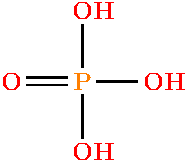
\includegraphics[scale=\modDGHyperImageScale] {\modInputPrefix/out/006_g_2_11311100.pdf}\\{$\mathrm{Phosphate}$}};
% id = 1, graphName = Cellobiose
\node[modStyleDGHyperVertex, at=(v-coord-1-0)] (v-1-0) {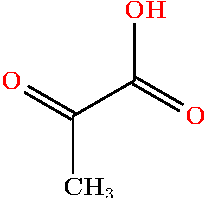
\includegraphics[scale=\modDGHyperImageScale] {\modInputPrefix/out/008_g_3_11311100.pdf}\\{$\mathrm{Cellobiose}$}};
% id = 2, graphName = p_{1,0}
\node[modStyleDGHyperVertex, at=(v-coord-2-0)] (v-2-0) {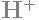
\includegraphics[scale=\modDGHyperImageScale] {\modInputPrefix/out/010_g_4_11311100.pdf}\\{$\mathrm{p_{1,0}}$}};
% id = 3, graphName = p_{1,1}
\node[modStyleDGHyperVertex, at=(v-coord-3-0)] (v-3-0) {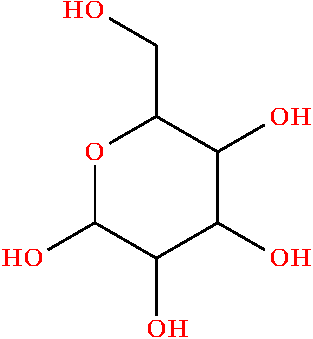
\includegraphics[scale=\modDGHyperImageScale] {\modInputPrefix/out/012_g_5_11311100.pdf}\\{$\mathrm{p_{1,1}}$}};
% id = 5, graphName = ATP
\node[modStyleDGHyperVertex, at=(v-coord-5-0)] (v-5-0) {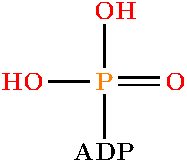
\includegraphics[scale=\modDGHyperImageScale] {\modInputPrefix/out/004_g_1_11311100.pdf}\\{$\mathrm{ATP}$}};
% id = 6, graphName = p_{2,0}
\node[modStyleDGHyperVertex, at=(v-coord-6-0)] (v-6-0) {
\includegraphics[scale=\modDGHyperImageScale] {\modInputPrefix/out/016_g_20_11311100.pdf}\\{$\mathrm{p_{2,0}}$}};
% id = 7, graphName = p_{2,1}
\node[modStyleDGHyperVertex, at=(v-coord-7-0)] (v-7-0) {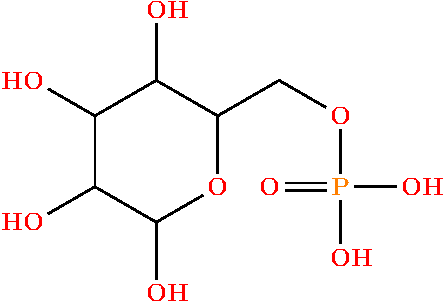
\includegraphics[scale=\modDGHyperImageScale] {\modInputPrefix/out/018_g_21_11311100.pdf}\\{$\mathrm{p_{2,1}}$}};
% id = 9, graphName = H2O
\node[modStyleDGHyperVertex, at=(v-coord-9-0)] (v-9-0) {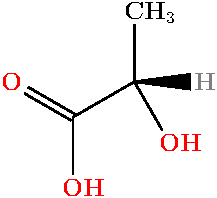
\includegraphics[scale=\modDGHyperImageScale] {\modInputPrefix/out/002_g_0_11311100.pdf}\\{$\mathrm{H2O}$}};
% id = 10, graphName = p_{3,0}
\node[modStyleDGHyperVertex, at=(v-coord-10-0)] (v-10-0) {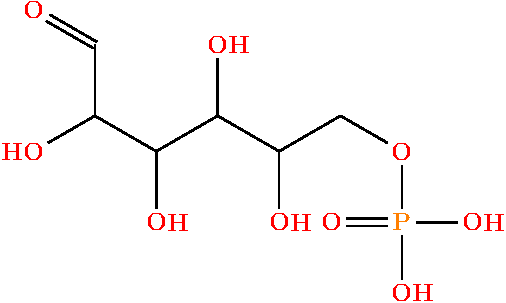
\includegraphics[scale=\modDGHyperImageScale] {\modInputPrefix/out/022_g_32_11311100.pdf}\\{$\mathrm{p_{3,0}}$}};
% id = 4{ 'Phosphate' 'Cellobiose' }, ' cellobiose + phosphate = alpha-D-glucose 1-phosphate + D-glucose', { 'p_{1,0}' 'p_{1,1}' }
\node[modStyleDGHyperEdge, at=(v-coord-4-0)] (v-4-0) {$\mathrm{r_{0}}$};
% id = 8{ 'ATP' 'p_{1,1}' }, ' ATP+glucose= ADP+Glucose 6-phosphate', { 'p_{2,0}' 'p_{2,1}' }
\node[modStyleDGHyperEdge, at=(v-coord-8-0)] (v-8-0) {$\mathrm{r_{1}}$};
% id = 4{ 'Phosphate' 'Cellobiose' }, ' cellobiose + phosphate = alpha-D-glucose 1-phosphate + D-glucose', { 'p_{1,0}' 'p_{1,1}' }
\path[modStyleDGHyperConnector] (v-0-0) to (v-4-0);
\path[modStyleDGHyperConnector] (v-1-0) to (v-4-0);
\path[modStyleDGHyperConnector] (v-4-0) to (v-2-0);
\path[modStyleDGHyperConnector] (v-4-0) to (v-3-0);
% id = 8{ 'ATP' 'p_{1,1}' }, ' ATP+glucose= ADP+Glucose 6-phosphate', { 'p_{2,0}' 'p_{2,1}' }
\path[modStyleDGHyperConnector] (v-3-0) to (v-8-0);
\path[modStyleDGHyperConnector] (v-5-0) to (v-8-0);
\path[modStyleDGHyperConnector] (v-8-0) to (v-6-0);
\path[modStyleDGHyperConnector] (v-8-0) to (v-7-0);
% id = 11{ 'p_{2,1}' }, ' glucose= D-Glucose ', { 'p_{3,0}' }
\path[modStyleDGHyperConnector] (v-7-0) to node[auto, swap] {$\mathrm{r_{5}}$} (v-10-0);
\end{tikzpicture}%
